\documentclass[11pt,a4paper,onecolumn,notitlepage]{article}


%!TEX root = proposal.tex
% Packages
\usepackage[show]{chato-notes}
\usepackage{url}
\usepackage{hyperref}
\usepackage{graphicx}
\usepackage{multirow}
\usepackage{amssymb}
\usepackage{amsmath}
\usepackage{centernot}
% avoid conflicts
\let\proof\relax
\let\endproof\relax
\usepackage{amsthm}
\usepackage{algorithm}
\usepackage{algorithmicx}
\usepackage[noend]{algpseudocode}
\usepackage{enumerate}
\usepackage[dvipsnames]{xcolor}
\usepackage{colortbl}
\usepackage[style=base]{caption}
\usepackage{subcaption}
\usepackage{comment}
\usepackage{balance}
\usepackage{cite} %citations are ordered by number
\usepackage[tikz]{bclogo}
\usepackage[normalem]{ulem}
\usepackage{tikz}
\usepackage{nccmath}
\usepackage{enumitem}
\usepackage{balance}
\usepackage{rotating}
\usepackage{pifont}
\usepackage[margin=2cm]{geometry}
\usepackage{etoolbox} % Patch the bibliography title
\usepackage[noindentafter]{titlesec}

\usetikzlibrary{decorations.markings}
%%
%% The next line says how the "vertex" style of nodes should look: drawn as small circles.
\tikzstyle{vertex}=[circle, draw, inner sep=0pt, minimum size=4pt, fill=black]
\newcommand{\vertex}{\node[vertex]}


\hypersetup{
%    bookmarks=true,         % show bookmarks bar?
    unicode=false,          % non-Latin characters in Acrobats bookmarks
    pdftoolbar=true,        % show Acrobats toolbar?
    pdfmenubar=true,        % show Acrobats menu?
    pdffitwindow=false,     % window fit to page when opened
    pdfstartview={FitH},    % fits the width of the page to the window
    pdftitle={My title},    % title
    pdfauthor={Author},     % author
    pdfsubject={Subject},   % subject of the document
    pdfcreator={Creator},   % creator of the document
    pdfproducer={Producer}, % producer of the document
    pdfnewwindow=true,      % links in new window
    colorlinks=true,       % false: boxed links; true: colored links
    linkcolor=black,          % color of internal links
    citecolor=black,        % color of links to bibliography
    filecolor=black,      % color of file links
    urlcolor=black,           % color of external links
}



\newcommand*{\graphpair}[2]{\langle #1, #2 \rangle}
\newcommand*{\tuple}[1]{(#1_1, ..., #1_n)}
\newcommand*{\range}[3]{#1 = #2 ... #3}
\newcommand*{\pair}[2]{(#1,#2)}
\newcommand*{\triple}[3]{(#1,#2,#3)}
\newcommand*{\edge}[4]{#1 \overset{#3}{#4} #2}
\newcommand*{\uedge}[2]{\edge{#1}{#2}{}{--}}
\newcommand*{\dedge}[2]{\edge{#1}{#2}{}{\rightarrow}}
\newcommand*{\luedge}[3]{\edge{#1}{#2}{#3}{--}}
\newcommand*{\ldedge}[3]{\edge{#1}{#2}{#3}{\rightarrow}}
\newcommand*{\expgname}[1]{#1^+}
\newcommand*{\expgraph}[3]{\expgname{#1}:\graphpair{#2^+}{#3^+}}


%Paper macros



%Style macros
\renewcommand\abstractname{Summary}
%\patchcmd{\thebibliography}{\section*}{\section}{}{}
\renewcommand{\refname}{Bibliography}

%% Work package styles (DO NOT touch)
\renewcommand\theparagraph{\Alph{paragraph}}
\renewcommand\thesubparagraph{[\Alph{paragraph}\arabic{subparagraph}]}
\titleformat{\paragraph}{\normalfont\large\bfseries}{\theparagraph}{1em}{}
\titleformat{\subparagraph}{\normalfont\normalsize\bfseries}{\thesubparagraph}{1em}{}
\titlespacing*{\subparagraph}{0pt}{3.25ex plus 1ex minus .2ex}{1.25ex plus .1ex}
\newcommand{\workpack}{\paragraph}
\newcommand{\subworkpack}{\subparagraph}

\setcounter{secnumdepth}{5}

%Algorithmic macros
\renewcommand{\algorithmicrequire}{\textbf{Input:}}
\renewcommand{\algorithmicensure}{\textbf{Output:}}
\renewcommand{\algorithmicforall}{\textbf{for each}}
\algdef{SE}[DOWHILE]{Do}{DoWhile}{\algorithmicdo}[1]{\algorithmicwhile\ #1}%

%Complexity macros
\newcommand*{\NP}{$\mathbf{NP}$}
\newcommand*{\NPhard}{$\mathbf{NP}$-hard}
\newcommand*{\NPcomplete}{$\mathbf{NP}$-complete}
\newcommand*{\SPcomplete}{$\mathbf{\#P}$-complete}
\newcommand*{\SPhard}{$\mathbf{\#P}$-hard}
\newcommand*{\bigO}{\mathcal{O}}

% Paragraphs
\newcommand{\spara}[1]{\smallskip\noindent{\bf #1}}
\newcommand{\mpara}[1]{\medskip\noindent{\bf #1}}
\newcommand{\para}[1]{\noindent{\bf #1}}

\newcommand{\blackBox}{$\blacksquare$}



\newcommand{\removed}[1]{
  \colorbox{red!30}{{\scriptsize REMOVED}}
  {\color{red}#1}
}

\newcommand{\del}[1]{
  {\color{red}\sout{#1}}
}


\newcommand{\added}[1]{
{\color{ForestGreen}#1}
}



\begin{document}
\title{Graph mining - WS 2016 - Project Report}



%\institute{}

\date{Due date: 24 January 2017}

\author{
Maxi Fischer, S\"oren Tietb\"ohl\\ 
}


\maketitle



% - Summary of the project
\begin{abstract}
Analysis of the Spotify Artist Network using an ego-based community detection algorithm.
\end{abstract}


\section{Summary of the data}

Spotify is a music streaming platform, hosting over 30 million songs and more than 2 million artists. The artists are associated with each other via the 'related artists' feature. This relation induces a graph, which is the subject of this project.

Because the related artists have to be queried one-by-one from the Spotify API we are only using a subset of the complete graph. Our subgraph is constructed by starting at an arbitrary artist (we chose the "Red Hot Chili Peppers") and then using breadth first traversal. The total number of nodes in the subgraph is 50992, the number of edges is 179425. The 'related artist' relation goes both ways, so its an undirected graph. We can assume that in reality the graph is dynamic, because new songs and thus artists will be added all the time. The nodes are not labelled, but various information on the artist relation can be requested, such as genre and popularity.

Degree Distribution: 
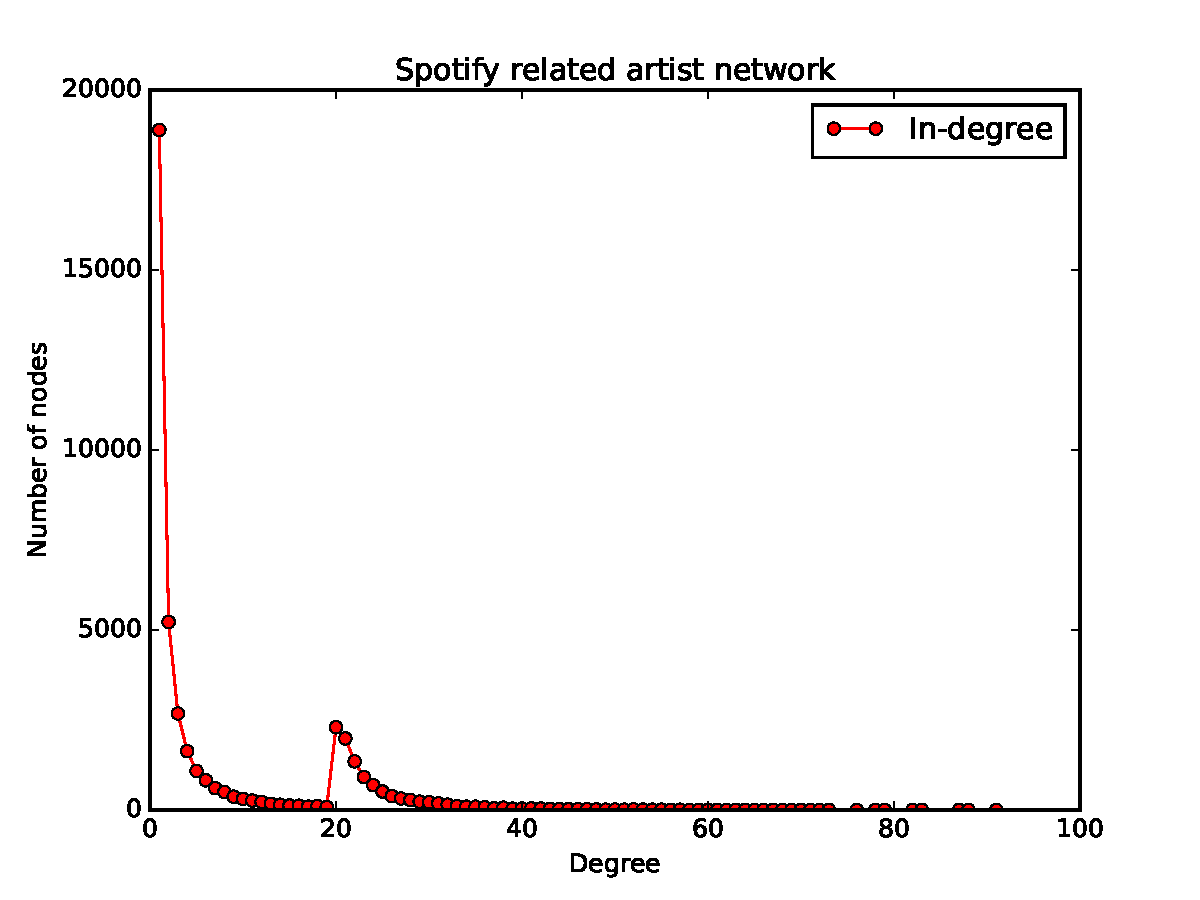
\includegraphics[scale=0.4]{spotify_degree_distribution.pdf}

The number of triangles is 913182. The average clustering coefficient is 0.2536.

\section{Description of the algorithm}

Our goal is the community detection in the graph to check the resulting communities against the genre distribution of the artists.

Therefore we chose two algorithms: the Louvain-algorithm\cite{louvain} and the k-Clique-Communities\cite{kclique}. For the Louvain algorithm we chose the best_partition function and for the k-Clique-Communities k = 2 to get the maximum number of partitions.

Briefly, the Louvain algorithms is a hierarchical clustering algorithm that greedy deletes edges that cause high modularity. In the resulting dendogram it chooses the best partition possible of the graph. The Louvain algorithm implementation takes a graph as an input and returns a dictionary with all nodes as keys and their community assignment as values. 

The k-Clique-Communities algorithm looks for all cliques of size k reachable by adjacent k-cliques. It takes the graph as an input and returns a list of sets of nodes, so the communities.

They are both usable on undirectional graphs.

\section{Preprocessing and storing}

In order to obtain the graph we queried the Spotify API at \cite{spotifyapi}. The related artist query returns 20 artists that are related to the given input artist.
From there we continued with breadth first traversal and queried the API for all the new artists. The graph is stored directly in main memory using python with networkx.
The nodes are named by the artists id on spotify, which is returned by the API.

Report all the preprocessing steps to obtain the final network. How do you store the data (graph database, main memory, disk)? In which format? Did you have to remove some information in order to clean the data? 

\section{Network analysis}

In this section, explain thoroughly the steps of the analysis you performed and give a motivation for such an analysis (e.g. discovering the most influential node, finding interesting patterns, analyzing communities). Elaborate on why you find it challenging and useful. Report possible applications.  

\subsection{Qualitative Results}

Comment the results of the analysis. You should also mention all the relevant details of your analysis, for instance specific values for parameters you used. It is preferable that you show some graphics and present some examples. If you use a visualization method to depict the nodes of the graph, make sure that you can explain at least a part of the network in the plot. 

For instance for node classification, show some of the classified vertices. If you have a ground truth, compare it to your results. You can also show a use case by running the algorithm on a smaller network (like the Star Wars network) and show what you find. 

For a graph query, show how the algorithm behaves with particular patterns (stars, triangles, cores ...).  Is the algorithm producing useful and interpretable results? Are the results unexpected or is it something you can find by yourself? Is there some anomaly?

\subsection{Time and scalability}

Evaluate the used method regarding its run time and scalability. Report the time you need to preprocess  the data (if there is such a phase, like an index construction) and to produce the results. On the same network and algorithm, consider incremental graph sizes (e.g. 10\% of the network, 30\%, etc.). 

\smallskip
\noindent Alternatively, generate some random network with \url{http://www.cse.ust.hk/graphgen/} or any other graph generator and compare the results of the algorithm between the two graphs (the original one and the random one). Are there any important differences in the outcome? Specify the parameters of the graph generator of choice. 


\subsection{[Optional] Memory usage}
Report how much memory is consumed by the algorithm. 


\section{Limitations and interesting findings}

Did you notice any limitation in the approach? Does it work as expected regarding the quality of the results? In terms of performance, is it too slow when the network is too big? Is it domain dependent or applicable to various types of graphs? To which kind of users are the results of the analysis useful? Describe what you have learned and propose ideas on how the analysis could improved. 



% - Bibliography
\bibliographystyle{abbrv}
\bibliography{bibliography}  

\end{document}
